% Replace this preamble with the official RLC 2026 template preamble (cover page disabled).
\documentclass{article}
\usepackage{graphicx,booktabs,amsmath,hyperref}
\graphicspath{{../outputs/figures/}}

\title{Which Improvements Transfer? Value-Based vs.\ Policy-Gradient Online Learning on ARC-AGI-3}
\author{Tebogo Seopa (2563912@students.wits.ac.za) \and Mandisa Mashinini (2589970@students.wits.ac.za)
  \and Onkabetse Monamodi (2854004@students.wits.ac.za)}

\begin{document}
\maketitle

\begin{abstract}
% Problem, approach, key quantitative result, main lesson. End with the public code link.
\end{abstract}

\section{Introduction}
% Problem, research question, contribution (matched, ablated comparison; not a new algorithm).

\section{Background and Related Work}
% DQN \cite{mnih2015dqn}, PPO \cite{schulman2017ppo}, count-based exploration \cite{bellemare2016count},
% DRQN / memory \cite{hausknecht2015drqn}, ARC-AGI-3 agents \cite{arcprize2026milestone1,smit2026goose}.

\section{Problem Formulation}
% POMDP: observation (64x64x16 one-hot, k-frame stack), action abstraction (6 + k^2, masked),
% reward (level delta; shaping is training-only), termination (WIN / GAME_OVER / budget), gamma.
% What persists between actions, levels, games, evaluation runs.

\section{Methods}
\subsection{DQN}
% Loss, replay, target network, epsilon schedule, masked max.
\subsection{PPO}
% Clipped surrogate, GAE, value loss, entropy, what is learned and when.
\subsection{Improvements}
% For each: observed limitation -> hypothesis -> intervention.

\section{Experimental Setup}
% Protocol (docs/PROTOCOL.md): splits, budget, seeds, hardware, hyperparameter table, package versions.

\section{Results}
% Table: official score, levels, wins, actions per version (mean +- std over 3 seeds), local vs Kaggle.
% \begin{tabular}{llrrrrrrrrrrr}
\toprule
run_name & split & seeds & score_mean & score_std & score_ci95 & levels_mean & levels_std & wins_mean & actions_mean & wall_time_s_mean & change_rate_mean & unique_states_mean \\
\midrule
dqn_baseline & dev & 3 & 0.11 & 0.18 & 0.20 & 1.67 & 0.58 & 0.00 & 15000.00 & 1423.64 & 0.67 & 5738.00 \\
dqn_imp1_explore & dev & 3 & 0.11 & 0.18 & 0.20 & 2.00 & 1.00 & 0.00 & 15000.00 & 1410.52 & 0.74 & 6577.00 \\
ppo_baseline & dev & 3 & 0.00 & 0.00 & 0.00 & 1.33 & 0.58 & 0.00 & 15000.00 & 494.39 & 0.68 & 5911.33 \\
ppo_imp1_explore & dev & 3 & 0.00 & 0.00 & 0.00 & 1.33 & 0.58 & 0.00 & 15000.00 & 1031.96 & 0.71 & 6356.00 \\
random & dev & 3 & 0.01 & 0.01 & 0.01 & 1.67 & 0.58 & 0.00 & 15000.00 & 55.45 & 0.68 & 5922.33 \\
\bottomrule
\end{tabular}

% Figure: learning curves per algorithm.
% 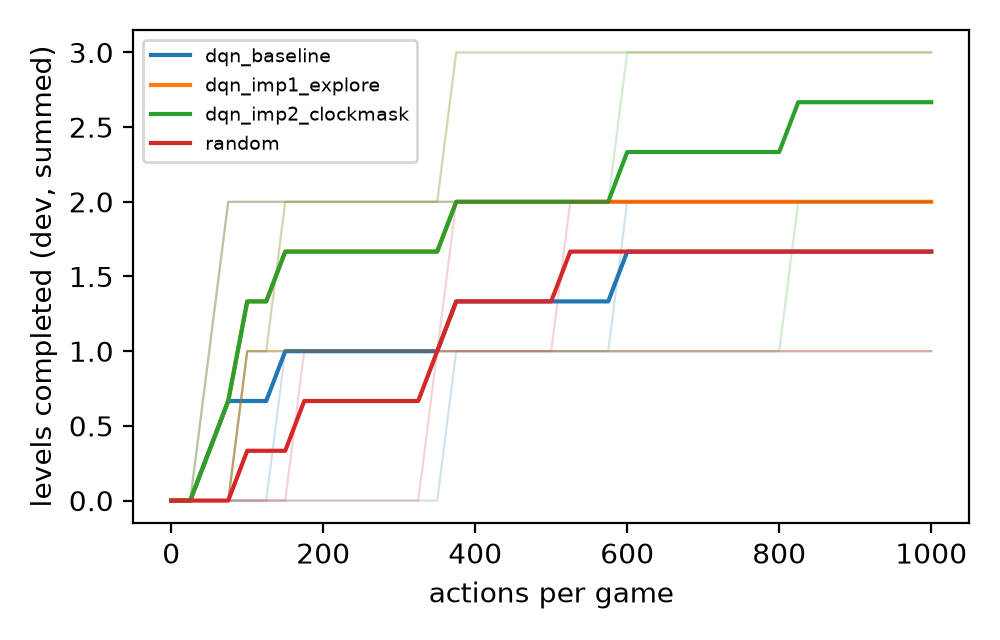
\includegraphics[width=\linewidth]{curve_dqn_dev.png}
\subsection{Ablations}
\subsection{Held-out Generalisation}
\subsection{Success and Failure Cases}

\section{Discussion and Limitations}
% Interaction efficiency, compute, what transferred across algorithms, what did not and why.

\section{Conclusion}

\bibliographystyle{plainnat}
\bibliography{refs}
\end{document}
